\documentclass[12pt]{article}
\usepackage[a4paper, margin=2cm, bottom=2cm]{geometry}
\usepackage{graphicx} % Required for inserting images
\usepackage{epstopdf}
\usepackage{minted}

\usepackage{tikz}
\usepackage{pgfplots}
\usepackage{pgfplotstable}
\usepackage{listings}
\usepackage{layouts}
% \usepackage[dvipsnames]{xcolor}

\usepackage[backend=biber]{biblatex}
\addbibresource{references.bib}

\usetikzlibrary{decorations.markings}
\usetikzlibrary{arrows.meta,pgfplots.units}
\usetikzlibrary{plotmarks,angles}
\usepgfplotslibrary{colorbrewer}
\usepgfplotslibrary{fillbetween}
\pgfplotsset{width=12cm}
\pgfplotsset{compat=1.18}

\usepackage{titling}
\usepackage[separate-uncertainty=true,multi-part-units=single]{siunitx}
\usepackage{amsmath, amssymb}
\usepackage{physics}
\usepackage{circuitikz}
\usepackage{makecell}
\usepackage{booktabs}
\usepackage{scalerel}
\usepackage{float}
\usepackage{multicol}
\usepackage{multirow}
\usepackage{titling}
\usepackage{subcaption}
\usepackage{bm}
\usepackage{nicefrac}
\usepackage{diagbox}

% \AtBeginDocument{\RenewCommandCopy\qty\SI}
\setminted{
    linenos=true,
    autogobble,
    breaklines=true
}
\newenvironment{longlisting}{\captionsetup{type=listing}}{}

\setlength{\droptitle}{-5em}

\usetikzlibrary{math}

\DeclareSIUnit\decade{decade}
\DeclareSIUnit\div{div}

\title{Week 2 Interim Report}
\author{Luca Owen-Jones \& Luka Pivovarsky}
\date{May 2026}

\begin{document}
\maketitle
\section{Exercise 1}
\subsection{\texttt{ueintbit.m} listing}
\begin{listing}[H]
    \centering
    \inputminted{matlab}{../ueintbit.m}
    \label{lst:ueintbit}
    \caption{\texttt{ueintbit.m}}
\end{listing}

\subsection{Script listing}
\begin{longlisting}
    \centering
    \inputminted{matlab}{../script1.m}
    \label{lst:script1}
    \caption{\texttt{script1.m}}
\end{longlisting}

\subsection{Momentum Thickness Plot}
\begin{figure}[H]
    \centering
    
\includegraphics[width=16cm]{../Figures/script1}
    \caption{Momentum thickness variation for a zero pressure gradient laminar boundary layer.}
    \label{fig:ex1}
\end{figure}

\section{Exercise 2}
\subsection{Script listing}
\begin{longlisting}
    \centering
    \inputminted{matlab}{../script2.m}
    \label{lst:script2}
    \caption{\texttt{script2.m}}
\end{longlisting}

\subsection{Tabulated separation points}


% Re_L = 5.0e+06, duedx = -0.10, transition location = 0.480000, Rethet = 1.080189e+03 
% Re_L = 5.0e+06, duedx = 0.00, transition location = 0.740000, Rethet = 1.290349e+03 
% Re_L = 5.0e+06, duedx = 0.10, no transition, Rethet = 1.405774e+03 
% Re_L = 1.0e+07, duedx = -0.10, transition location = 0.290000, Rethet = 1.168598e+03 
% Re_L = 1.0e+07, duedx = 0.00, transition location = 0.370000, Rethet = 1.290349e+03 
% Re_L = 1.0e+07, duedx = 0.10, transition location = 0.550000, Rethet = 1.514451e+03 
% Re_L = 2.0e+07, duedx = -0.10, transition location = 0.170000, Rethet = 1.253209e+03 
% Re_L = 2.0e+07, duedx = 0.00, transition location = 0.190000, Rethet = 1.307670e+03 
% Re_L = 2.0e+07, duedx = 0.10, transition location = 0.220000, Rethet = 1.384823e+03
\sisetup{
round-mode = places,
round-precision = 2
}
\begin{table}[H]
    \centering
    \begin{tabular}{S[round-mode = none]cccccc}
        \toprule
        {\multirow{3}{*}{$\frac{\dd{u_e / U}}{\dd{x/L}}$}} & \multicolumn{6}{c}{$\mathrm{Re}_L$} \\ \cmidrule(lr){2-7}
         & \multicolumn{2}{c}{\num{5e6}} & \multicolumn{2}{c}{\num{1e7}} & \multicolumn{2}{c}{\num{2e7}} \\ \cmidrule(lr){2-3} \cmidrule(lr){4-5} \cmidrule(lr){6-7}
         & {$x_\mathrm{tr}/L$} & {$\mathrm{Re}_\theta$} & {$x_\mathrm{tr}/L$} & {$\mathrm{Re}_\theta$} & {$x_\mathrm{tr}/L$} & {$\mathrm{Re}_\theta$} \\ \midrule
         -0.1 & \num{0.480000} & \num{1.080189e+03} & \num{0.290000} & \num{1.168598e+03} & \num{0.170000} & \num{1.253209e+03} \\
         0 & \num{0.740000} & \num{1.290349e+03} & \num{0.370000} & \num{1.290349e+03} & \num{0.190000} & \num{1.307670e+03} \\
         0.1 & --- & --- & \num{0.550000} & \num{1.514451e+03} & \num{0.220000} & \num{1.384823e+03} \\
         \bottomrule
    \end{tabular}
    \caption{Transition locations and $\mathrm{Re}_\theta$ locations for a constant velocity gradient laminar boundary layer.}
    \label{tab:transition_locations}
\end{table}

\section{Exercise 3}
\subsection{Script listing}
\begin{longlisting}
    \centering
    \inputminted{matlab}{../script3.m}
    \label{lst:script3}
    \caption{\texttt{script3.m}}
\end{longlisting}

\section{Exercise 5}
\subsection{Script listing}
\begin{longlisting}
    \centering
    \inputminted{matlab}{../script5.m}
    \label{lst:script5}
    \caption{\texttt{script5.m}}
\end{longlisting}

\subsection{Graph}
\begin{figure}[H]
    \centering
    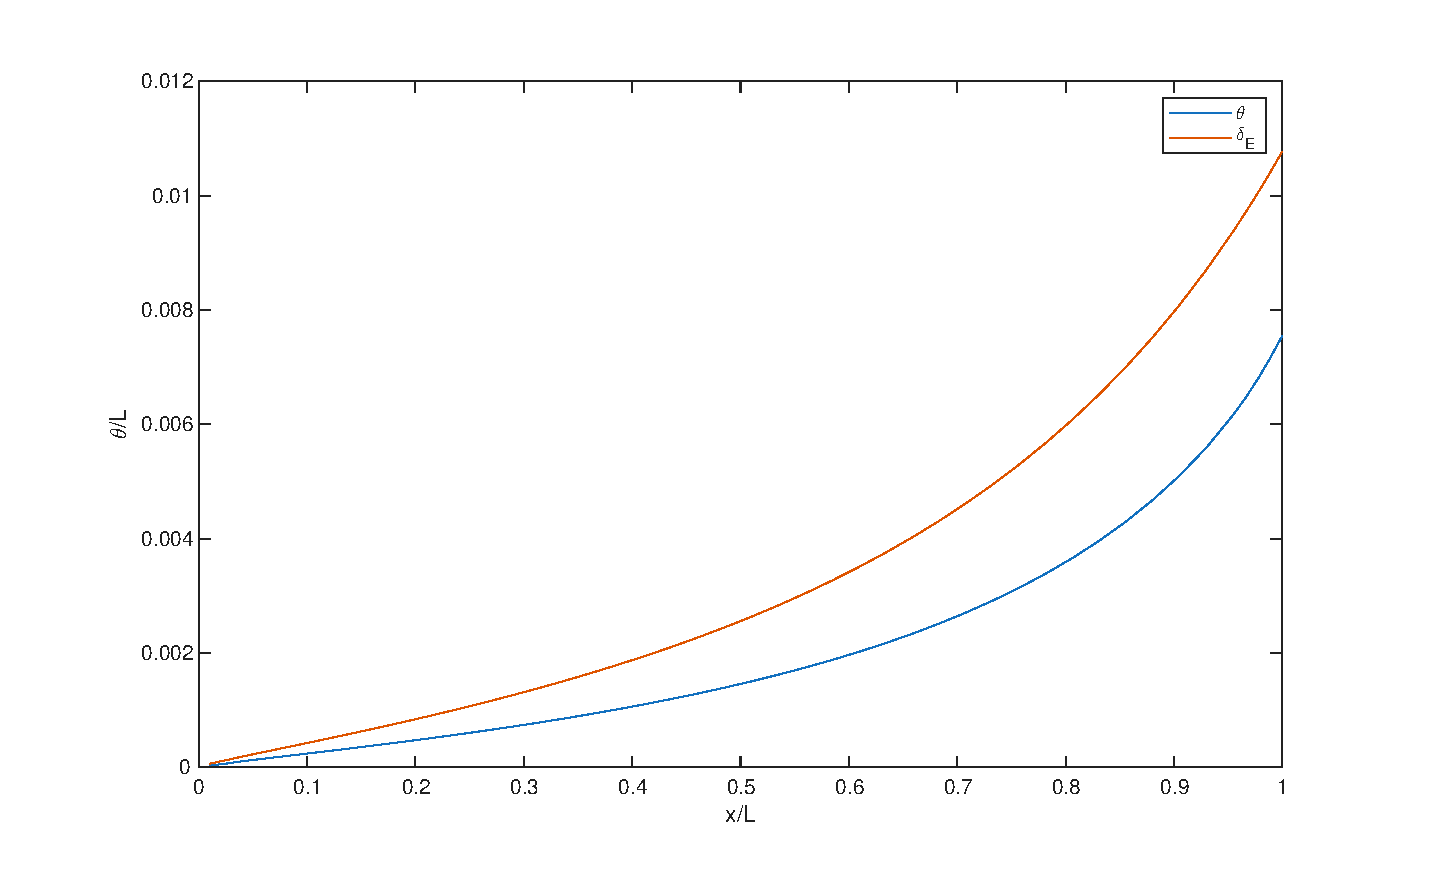
\includegraphics[width=16cm]{../Figures/script5}
    \caption{Surface velocity versus fractional angle for zero incidence.}
    \label{fig:week5.3}
\end{figure}

\section{Exercise 6}
\subsection{Script listing}
\begin{longlisting}
    \centering
    \inputminted{matlab}{../script6.m}
    \label{lst:script5}
    \caption{\texttt{script6.m}}
\end{longlisting}

\subsection{Plots}
\printinunitsof{cm}\prntlen{\textwidth}
\begin{figure}[H]
    \centering
    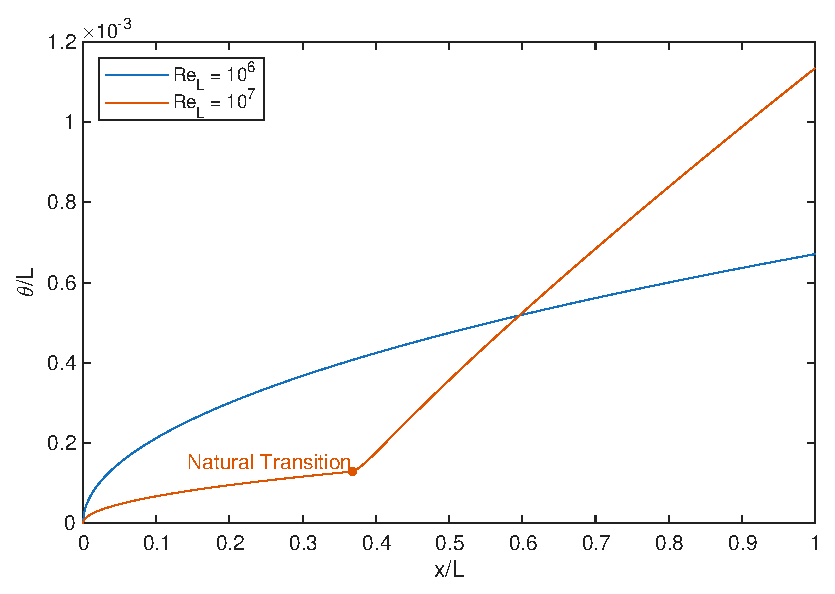
\includegraphics[width=16cm]{../Figures/script6_theta1}
    \caption{Surface velocity versus fractional angle for zero incidence.}
    \label{fig:week5_theta1}
\end{figure}
\begin{figure}[H]
    \centering
    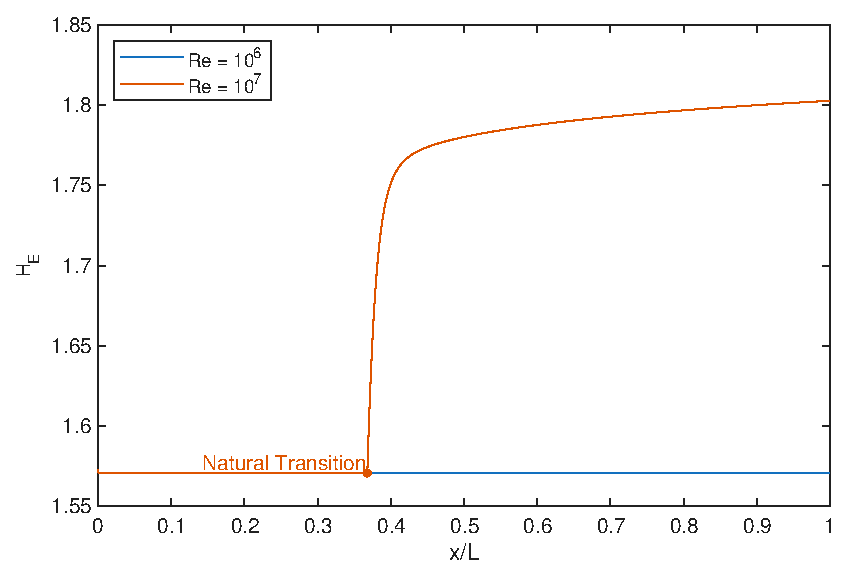
\includegraphics[width=16cm]{../Figures/script6_he1}
    \caption{Surface velocity versus fractional angle for zero incidence.}
    \label{fig:week5.3}
\end{figure}
\begin{figure}[H]
    \centering
    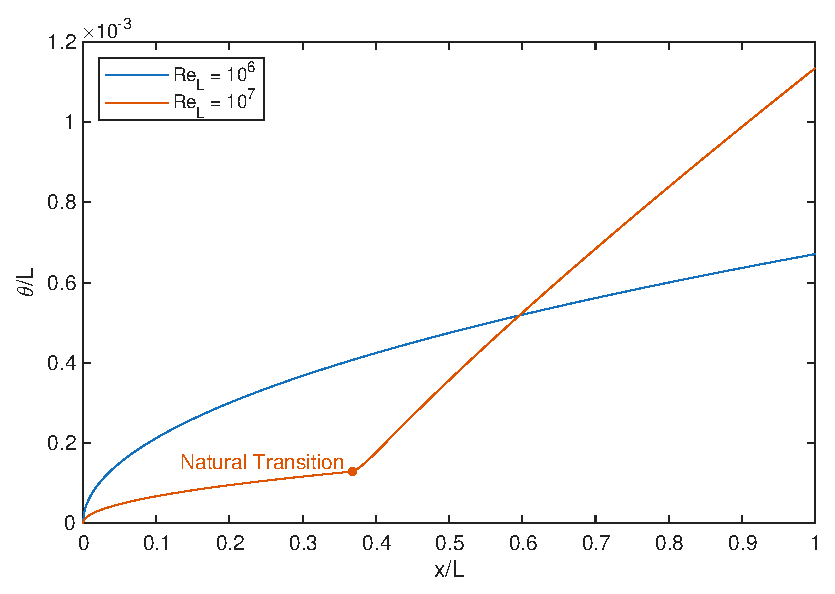
\includegraphics[width=16cm]{../Figures/script6_theta2}
    \caption{Surface velocity versus fractional angle for zero incidence.}
    \label{fig:week5_theta1}
\end{figure}
\begin{figure}[H]
    \centering
    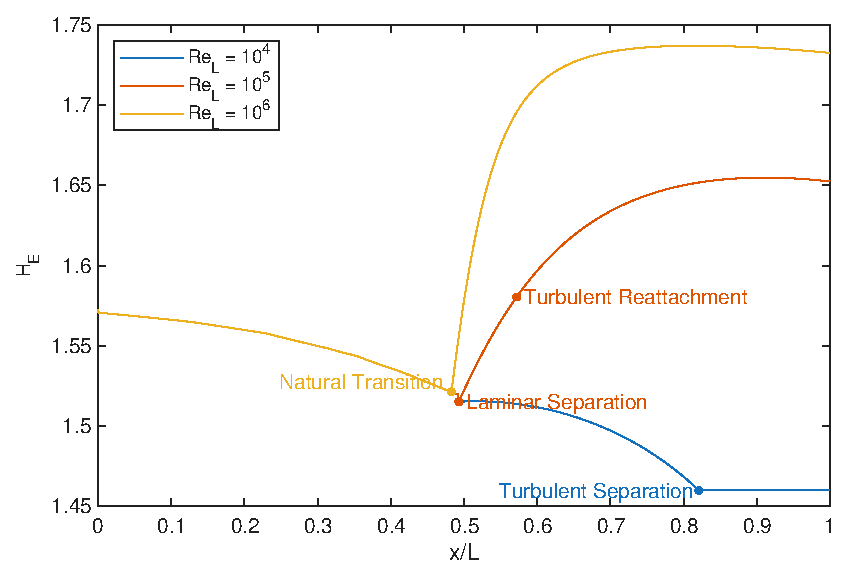
\includegraphics[width=16cm]{../Figures/script6_he2}
    \caption{Surface velocity versus fractional angle for zero incidence.}
    \label{fig:week5.3}
\end{figure}
\end{document}